\documentclass{optica-article}
\journal{opticajournal} % for journals or Optica Open
\articletype{Research Article}
\usepackage{lineno}
\usepackage{verbatim}
\usepackage{graphicx} %immagini ecc
\usepackage{float}
\usepackage{hyperref}

\begin{document}

\title{ \begin{huge}
\textbf{Relazione Tecnica NAO Challenge23} 
\end{huge} }

\author{\centering NaoNexus}

\bigskip
\noindent
\textbf{PER MAGGIORI INFORMAZIONI:} \\

\noindent\textit{Visita il nostro} \href{https://www.naonexus.altervista.org/naochallenge2023/index.html}{sito}



\noindent \textit{Visita la nostra} \href{https://github.com/NaoNexus/ChallengeNao23}{repository}

\noindent\textit{Scrivi una email a: }\email{socialnaonexus@gmail.com}

\bigskip

\begin{figure}
    \centering
    
\includegraphics[scale=0.05]{figures/logo.png}
    \label{fig:logo_con_scritta}
\end{figure}

\tableofcontents

\vspace{10pt}

\newpage

\begin{abstract*} 
\vspace{7pt}
\noindent
\\Nella \emph{NAO Challenge} di quest'anno è stato scelto di sviluppare due progetti orientati alla sostenibilità ed energia green. La \emph{missione} del team è di avvicinare le persone alla sostenibiltà rendendola più accessibile e facilmente comprensibile. Questi progetti introducono le persone nel mondo dell'energia solare ed il loro scopo è di prevenire sprechi di energia in grandi strutture.\\

\section{METODOLOGIA E TECNICHE USATE}\label{sec:methodology_technologies}
Essendo un gruppo numeroso c'era la necessità di tenere traccia dei \emph{tasks} e tenere ogni componente al passo con l'ultima versione del software sviluppato. Per raggiungere questo scopo il team ha sfruttato due importanti tecnologie: \emph{GitHub} e \emph{Notion}.

\subsection{DevOps con Notion e metodologia Agile}\label{sec:devops_notion}
Per lavorare al progetto e tenere traccia del progresso il team ha usato \emph{Notion}, una piattaforma collaborativa per la gestione di note. Il termine \emph{DevOps} proviene da \emph{software development} e \emph{technology operations}, ed è costituito dai vari metodi che hanno scopo di migliorare la collaborazione \emph{end-to-end}. La web-app Notion presenta molti strumenti come gestione di task, tracciamento andamento progetto e liste to-do e grazie ad essi ogni componente del team è stato al corrente degli incarichi da portare a termine ad ogni appuntamento. Questa piattaforma di collaborazione integra wiki e database creando uno spazio di lavoro per gestione di dati e task. I progetti sono stati gestiti con la metodologia \emph{Agile}: i compiti principali sono stati divisi in sub-tasks per essere poi distribuiti tra i membri del team; questo ha portato ad una maggiore efficenza nello sviluppo del software.

\subsection{GitHub}\label{sec:git_hub}
GitHub è uno strumento importante che ha aiutato il team a salvare e gestire il codice. È una piattaforma cloud-based di hosting di respository Git che aiuta i membri a tenere traccia dei cambiamenti fatti nel codice grazie al controllo versione.\\
Attraverso il \emph{branching} e \emph{merging} ogni membro è stato capace di lavorare in modo sicuro sul codice evitando di intaccare direttamente la versione principale. Tutte le modifiche apportate sono tracciate e possono essere annullate nel caso portino ad errori.

\bigskip

\noindent
\textbf{I DUE PROGETTI}

\bigskip
\noindent
Il primo progetto vede NAO come un \emph{assistente} in un edificio. NAO è connesso ad un telefono grazie ad un \hyperref[sec:domotics_server]{server HTTP}. Gli utenti possono connettere lo smartphone al server ed inviare dati dell'ambiente scelto rilevati grazie ad un \hyperref[sec:domotics_sensor]{sensore}. Quando NAO riceve questi dati controlla la \hyperref[sec:domotics_domotics_server]{domotica} dell'edificio accendendo e spegnendo le \emph{luci}, alzando e abbassando le \emph{tapparelle} o accendendo e spegnendo il \emph{riscaldamento}.\\

%\bigskip
%\vspace{10pt}

\vspace{7pt}
\noindent
Il secondo progetto prevede la collaborazione con un'azienda esterna e il team ha collaborato con \emph{Amperia}, la quale punta a rendere la transizione green più efficente e semplice. Connettendo NAO al sito \emph{SolarEdge} (una piattaforma che consente di progettare installazioni di pannelli fotovoltaici) attraverso un \hyperref[sec:solaedge_server]{server HTTP} l'utente viene guidato nella compilazione del sito che crea questo progetto.\\

\end{abstract*}

%%%%%%%%%%%%%%%%%%%%%%%%%%  body  %%%%%%%%%%%%%%%%%%%%%%%%%%

\section{NAO COME AIUTANTE DOMOTICO}\label{sec:domotics_project}
Questo progetto comprende che NAO comunichi con un \hyperref[sec:domotics_sensor]{sensore} per riuscire a ricavare le condizioni ambientali e sulla base di queste misurazioni controlla il 
server della \hyperref[sec:domotics_domotics_server]{domotica}. Il progetto si sviluppa su più step: inizialmente i dati vengono misurati con il \hyperref[sec:domotics_sensor]{sensore}, il PDF generato viene poi selezionato con l'\hyperref[sec:domotics_app]{app} sviluppata. Questi dati vengono poi inviati al \hyperref[sec:domotics_server]{server} insieme al numero di persone presenti nella stanza, che viene inserito direttamente sull'app. Questi dati vengono inviati a \hyperref[sec:domotics_nao]{NAO}, il quale manda i comandi alla domotica se specifici limiti sono sorpassati. Il progetto presenta vari elementi:\\

\begin{itemize}
    \item \hyperref[sec:domotics_sensor]{Sensore}: dispositivo esterno che misura dati ambientali ed esporta i risultati su un PDF;
    \item \hyperref[sec:domotics_app]{App}: una app che legge il PDF e lo invia al server HTTP insieme al numero di persone presenti nella stanza e alla luce interna;
    \item \hyperref[sec:domotics_server]{HTTP Server}: un server Rest che consente di visualizzare i dati estratti dal PDF tramite pagine web e comunica con il server della domotica;
    \item \hyperref[sec:domotics_nao]{NAO}: il robot umanoide che ricava i dati dal server e controlla la domotica sulla base di questi dati, comunicando inoltre i dati ricavati all'utente.
\end{itemize}.

\begin{figure}[H]
    \centering
    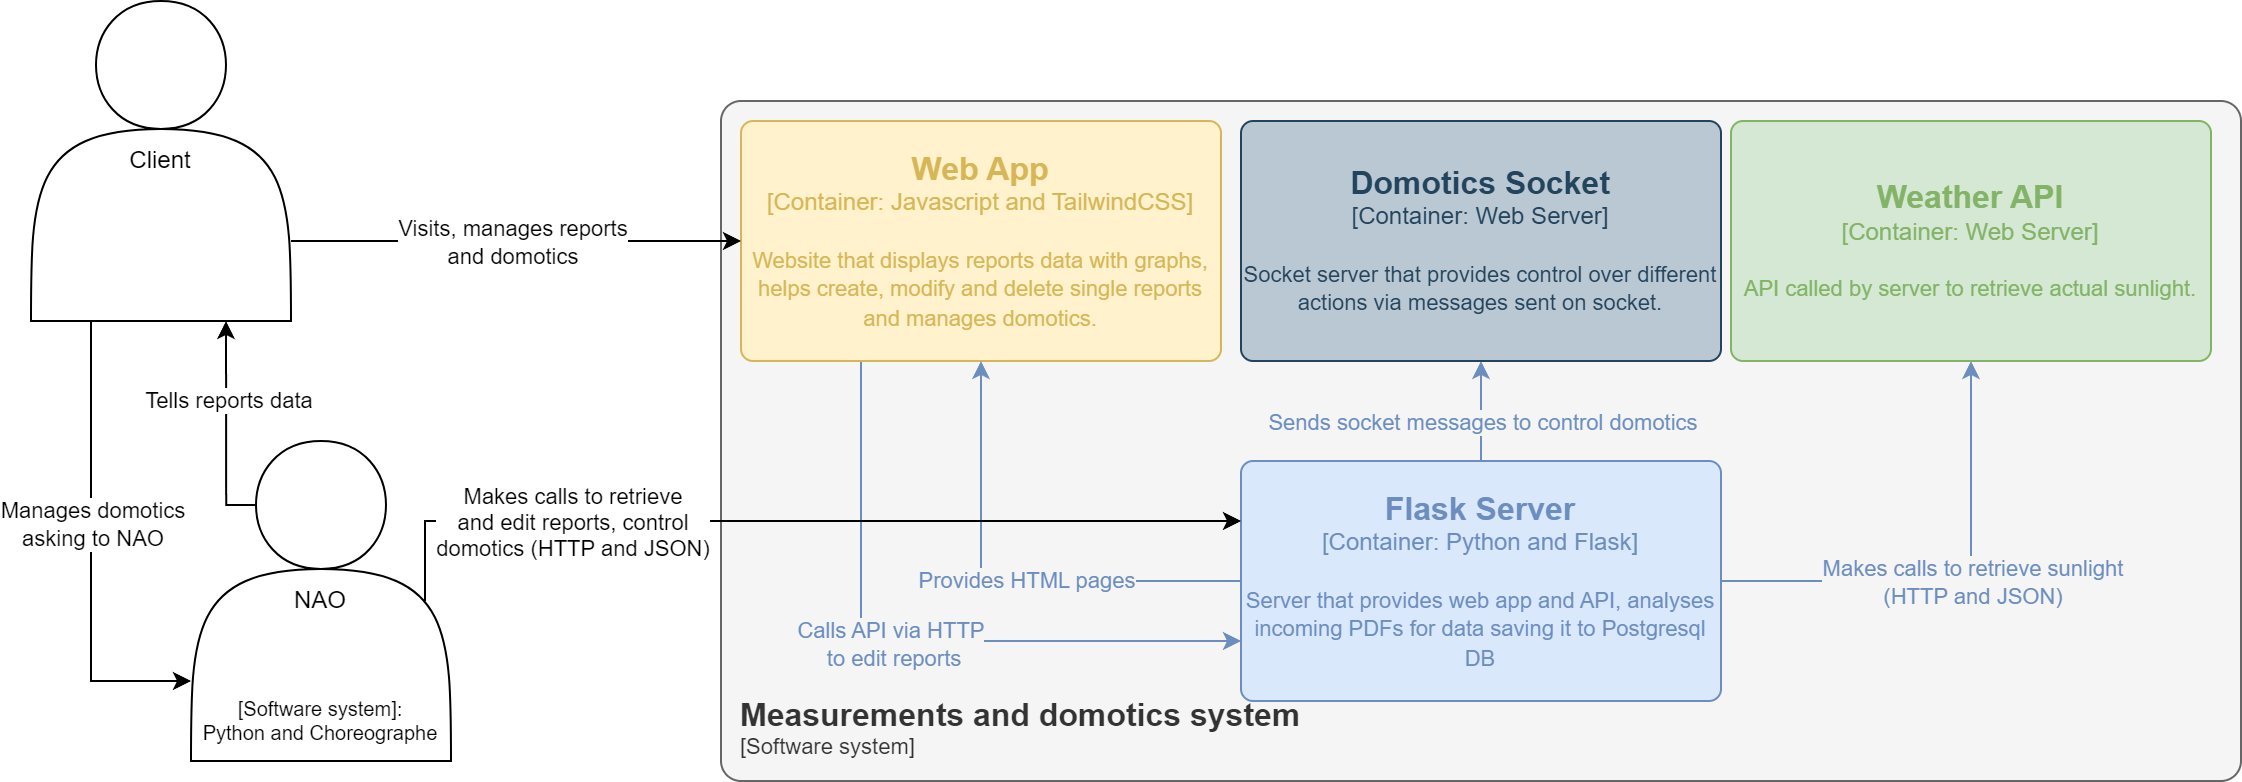
\includegraphics[scale=0.17]{figures/architecture_domotics.png}
    \caption{architettura software NAO domotica}
    \label{fig:my_label}
\end{figure}

\bigskip
\subsection{Il sensore}\label{sec:domotics_sensor}
\vspace{5pt}
Una parte significativa del progetto era quella di riuscire a ricavare ed analizzare i dati della concentrazione di CO2, temperatura e umidità dell'ambiente selezionato. In un primo momento si pensò di usare un Arduino da connettere al \hyperref[sec:domotics_server]{server HTTP}. Durante lo sviluppo del software il team ha incontrato molti problemi ed è stato deciso di comprare un sensore. Questo ha garantito risultati più precisi, i quali però vengono esportati in un file PDF.\\
\\Per analizzare i valori c'era il bisogno di avere un dispositivo che ricavasse i dati inviandoli al server. In un primo momento il team decise di connettere il sensore direttamente in una delle USB di NAO ma senza i permessi root gli archivi esterni non possono essere montati sull'umanoide, rendendo impossibile l'accesso a qualsiasi memoria esterna da NAO. E' stato quindi deciso di usare una \hyperref[sec:domotics_app]{app} per smartphone.\\

\bigskip
\subsection{L' App}\label{sec:domotics_app}
\vspace{5pt}
Questa app viene usata per caricare i PDF e mandarli al server. E' stata creata in quanto non c'era alcun modo per connettere il \hyperref[sec:domotics_sensor]{sensore} direttamente al server. Questo device manda i dati del sensore al server aggiungendo altre misurazioni utili che esso non può effettuare. Questa applicazione è stata scritta in \emph{Flutter} per renderla cross-platform e flessibile. Include un file picker e un input per inserire il \emph{numero di persone} in una stanza. Nel momento in cui viene inviato il file viene aggiunto alla richiesta il valore della \emph{luce} misurato con il sensore del telefono. L'applicazione inoltre elenca tutti i dati conservati nel \hyperref[sec:domotics_server]{server}.\\

\begin{figure}[H]
    \centering
    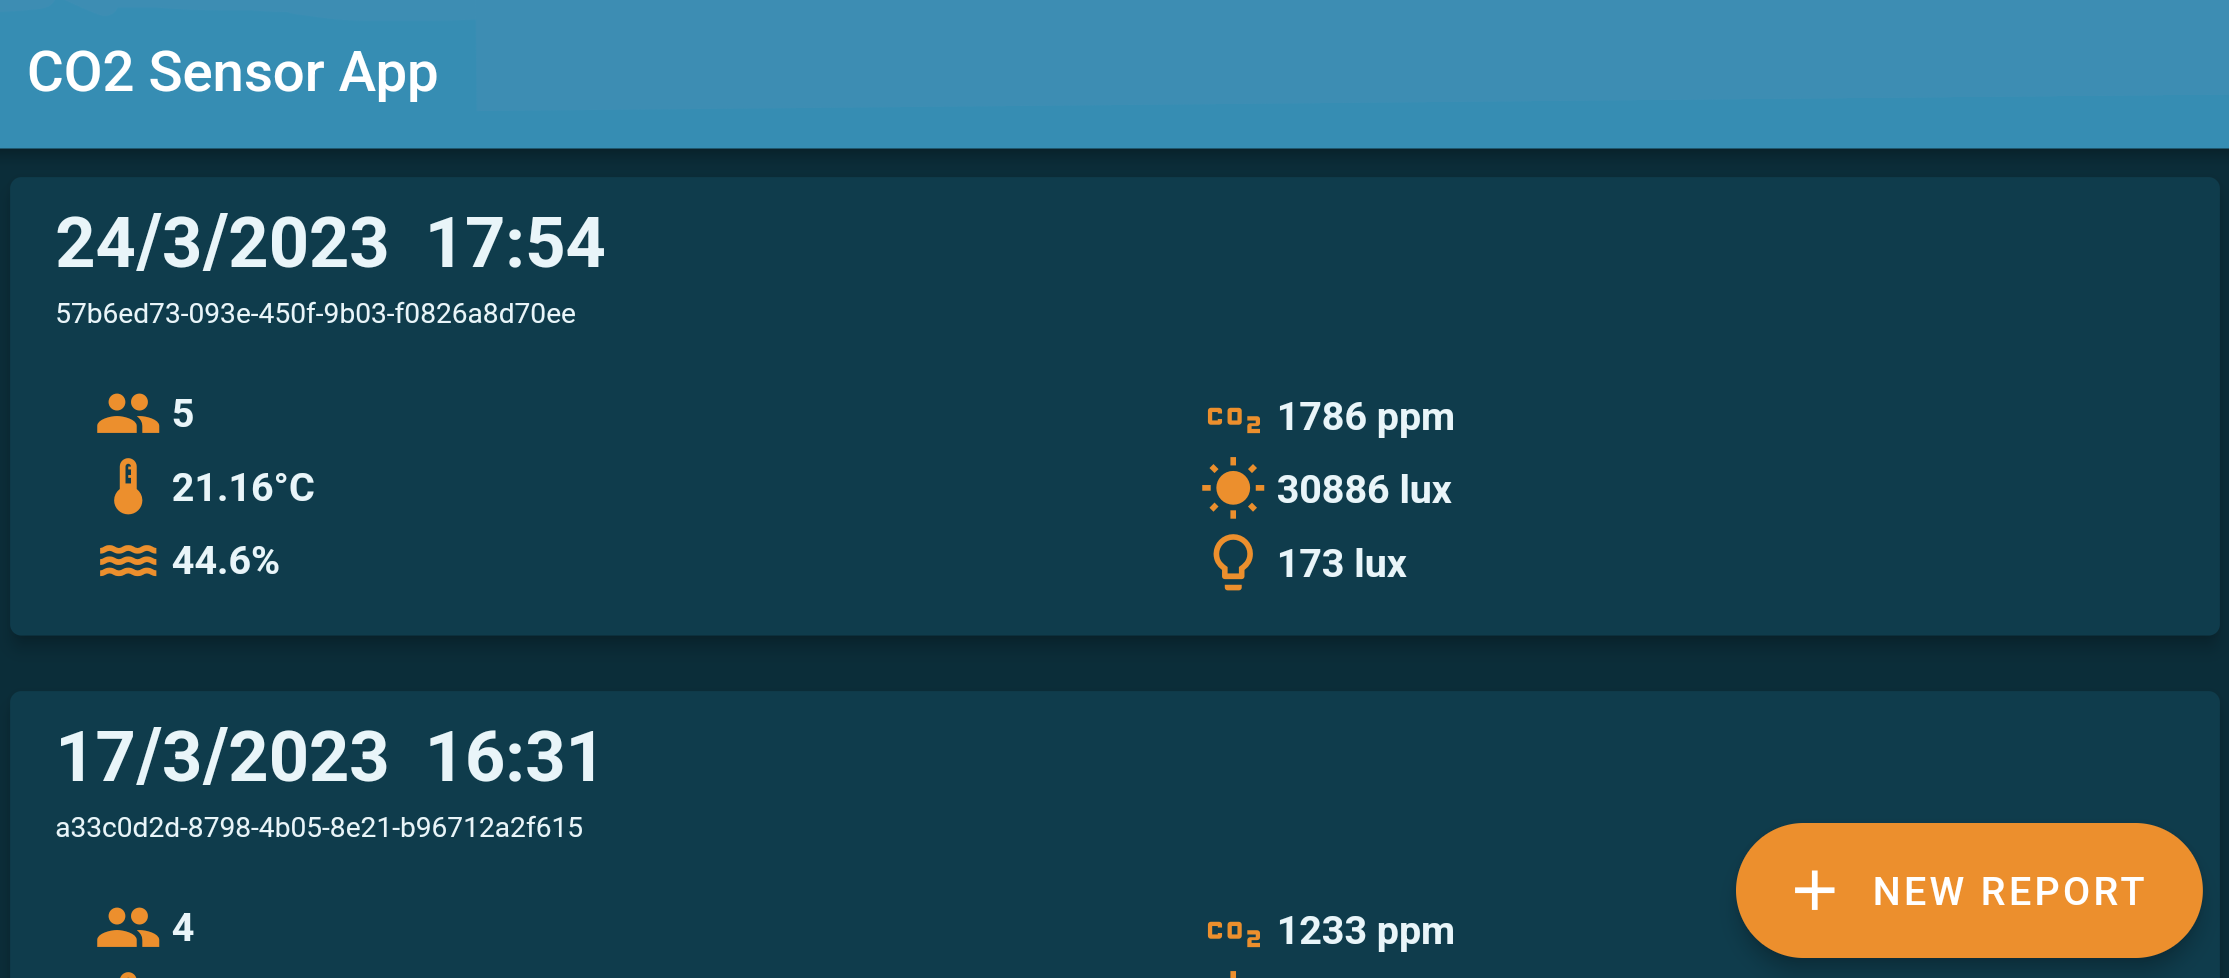
\includegraphics[scale=0.17]{figures/domotics_app.png}
    \caption{Applicazione domotica}
    \label{fig:app_domotica}
\end{figure}


\subsection{NAO}\label{sec:domotics_nao}
NAO è la parte centrale del progetto. È connesso al \hyperref[sec:domotics_server]{server HTTP} e riceve e salva i dati dell'ambiente selezionato, i quali sono usati da NAO per capire le chiamate da fare al server. Con il \hyperref[sec:domotics_domotics_server]{controllo domotico}, NAO dice all'utente cosa sta facendo. Il robot ha una funzionalità che permette di farlo diventare uno "smart home speaker" come \emph{"Alexa"}: l'end-user può chiedere a NAO di apportare modifiche alla domotica controllandola direttamente. Quando vengono ricevuti nuovi dati, NAO li comunica all'utente e basandosi su vari \emph{thresholds} può controllare gli smart devices.

\vspace{12pt}
\subsection{HTTP Server}\label{sec:domotics_server}
È il punto centrale in cui tutti i dati del progetto sono gestiti, è una parte del codice molto complessa scritta in Python, la quale \hyperref[sec:domotics_pdf_analysis]{analizza PDF}, aggiunge informazioni mancanti, presenta una \hyperref[sec:domotics_web_app]{Web App} che visualizza e gestisce dati e ha al suo interno la \hyperref[sec:domotics_rest_api]{Rest API} per connettere tutti i client come l' \hyperref[sec:domotics_app]{app} e \hyperref[sec:domotics_nao]{NAO}. L'idea iniziale era di eseguire il server su NAO ma le ultime versioni del software hanno rimosso la possibilità di entrare come utente \emph{root} e di installare pacchetti Python. È stato successivamente deciso di eseguire il server su un  \emph{Raspberry PI} con un \emph{IP statico} per renderlo accessibile da ogni client nella rete.

%serve tarduzione fixed IP - IP Statico - Grazie :)

\subsubsection{Web App}\label{sec:domotics_web_app}
Una parte importante del server è la web app che viene servita da esso: le pagine \emph{HTML} sono popolate utilizzando \href{https://jinja.palletsprojects.com/en/3.1.x/}{Jinja} e sono inviate usando \href{https://flask.palletsprojects.com/en/2.2.x/}{Flask}. Questa libreria è reponsabile del funzionamento del \hyperref[sec:domotics_rest_api]{server Rest} che distribuisce i dati anche in formato \emph{JSON}. In questa web app i dati dei report sono visualizzabili sotto forma di \emph{grafico} o \emph{lista}. Ogni report è \emph{modificabile} ed \emph{eliminabile}; è anche possibile \emph{aggiungere nuovi report} direttamente dall'UI. 

\begin{figure}[H]
    \centering
    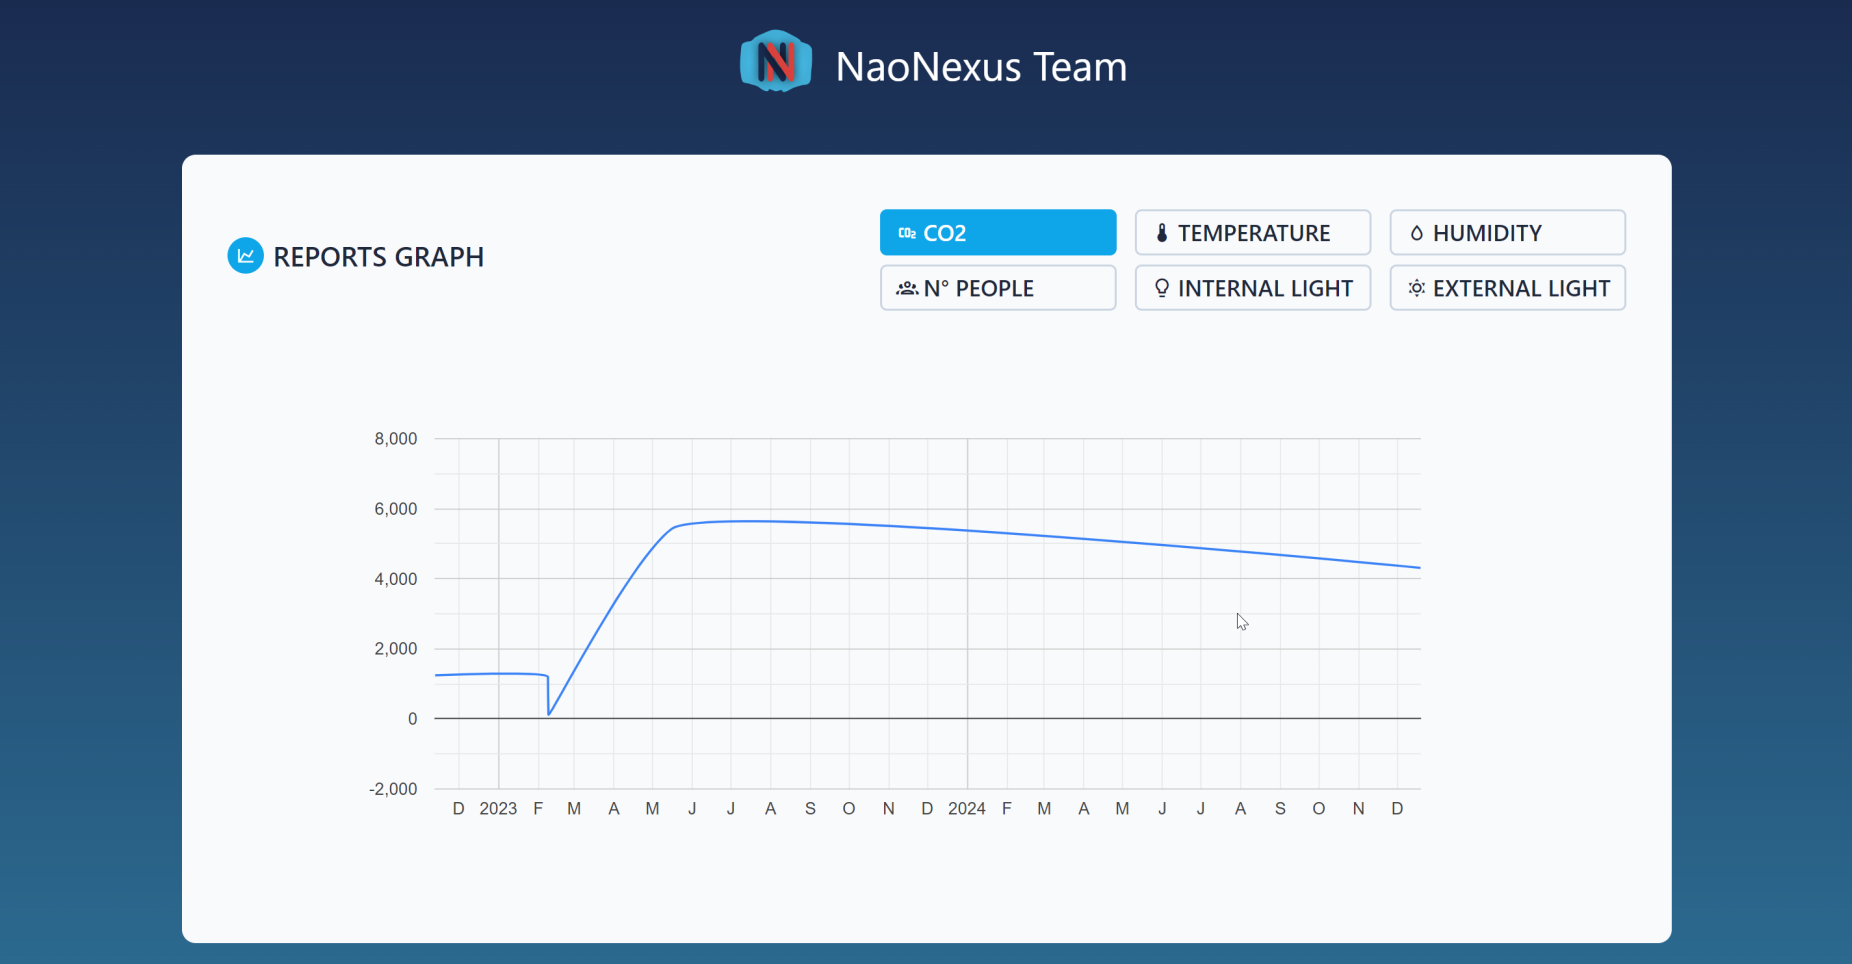
\includegraphics[scale=0.26]{figures/web_app_summary.png}
    \caption{Schermata con il riassunto dei report}
    \label{fig:webb_app_summary}
\end{figure}

\vspace{8pt}
\subsubsection{Rest API}\label{sec:domotics_rest_api}
\textit{La documentazione per l'API può essere trovata \href{https://naonexus.notion.site/Domotics-server-22721767d69a43a6badeafcaf546b3d2}{qui}.}\\
\\Il servizio Rest facilita lo scambio di dati tra tutti i client connessi, i quali sono poi inviati con \emph{JSON} usando \emph{HTTP} e sono accessibili poi tramite diversi endpoints. Il server Rest è scritto in  \href{https://flask.palletsprojects.com/en/2.2.x/}{Flask} come la \hyperref[sec:domotics_web_app]{web app}.


\begin{figure}[H]
    \centering
    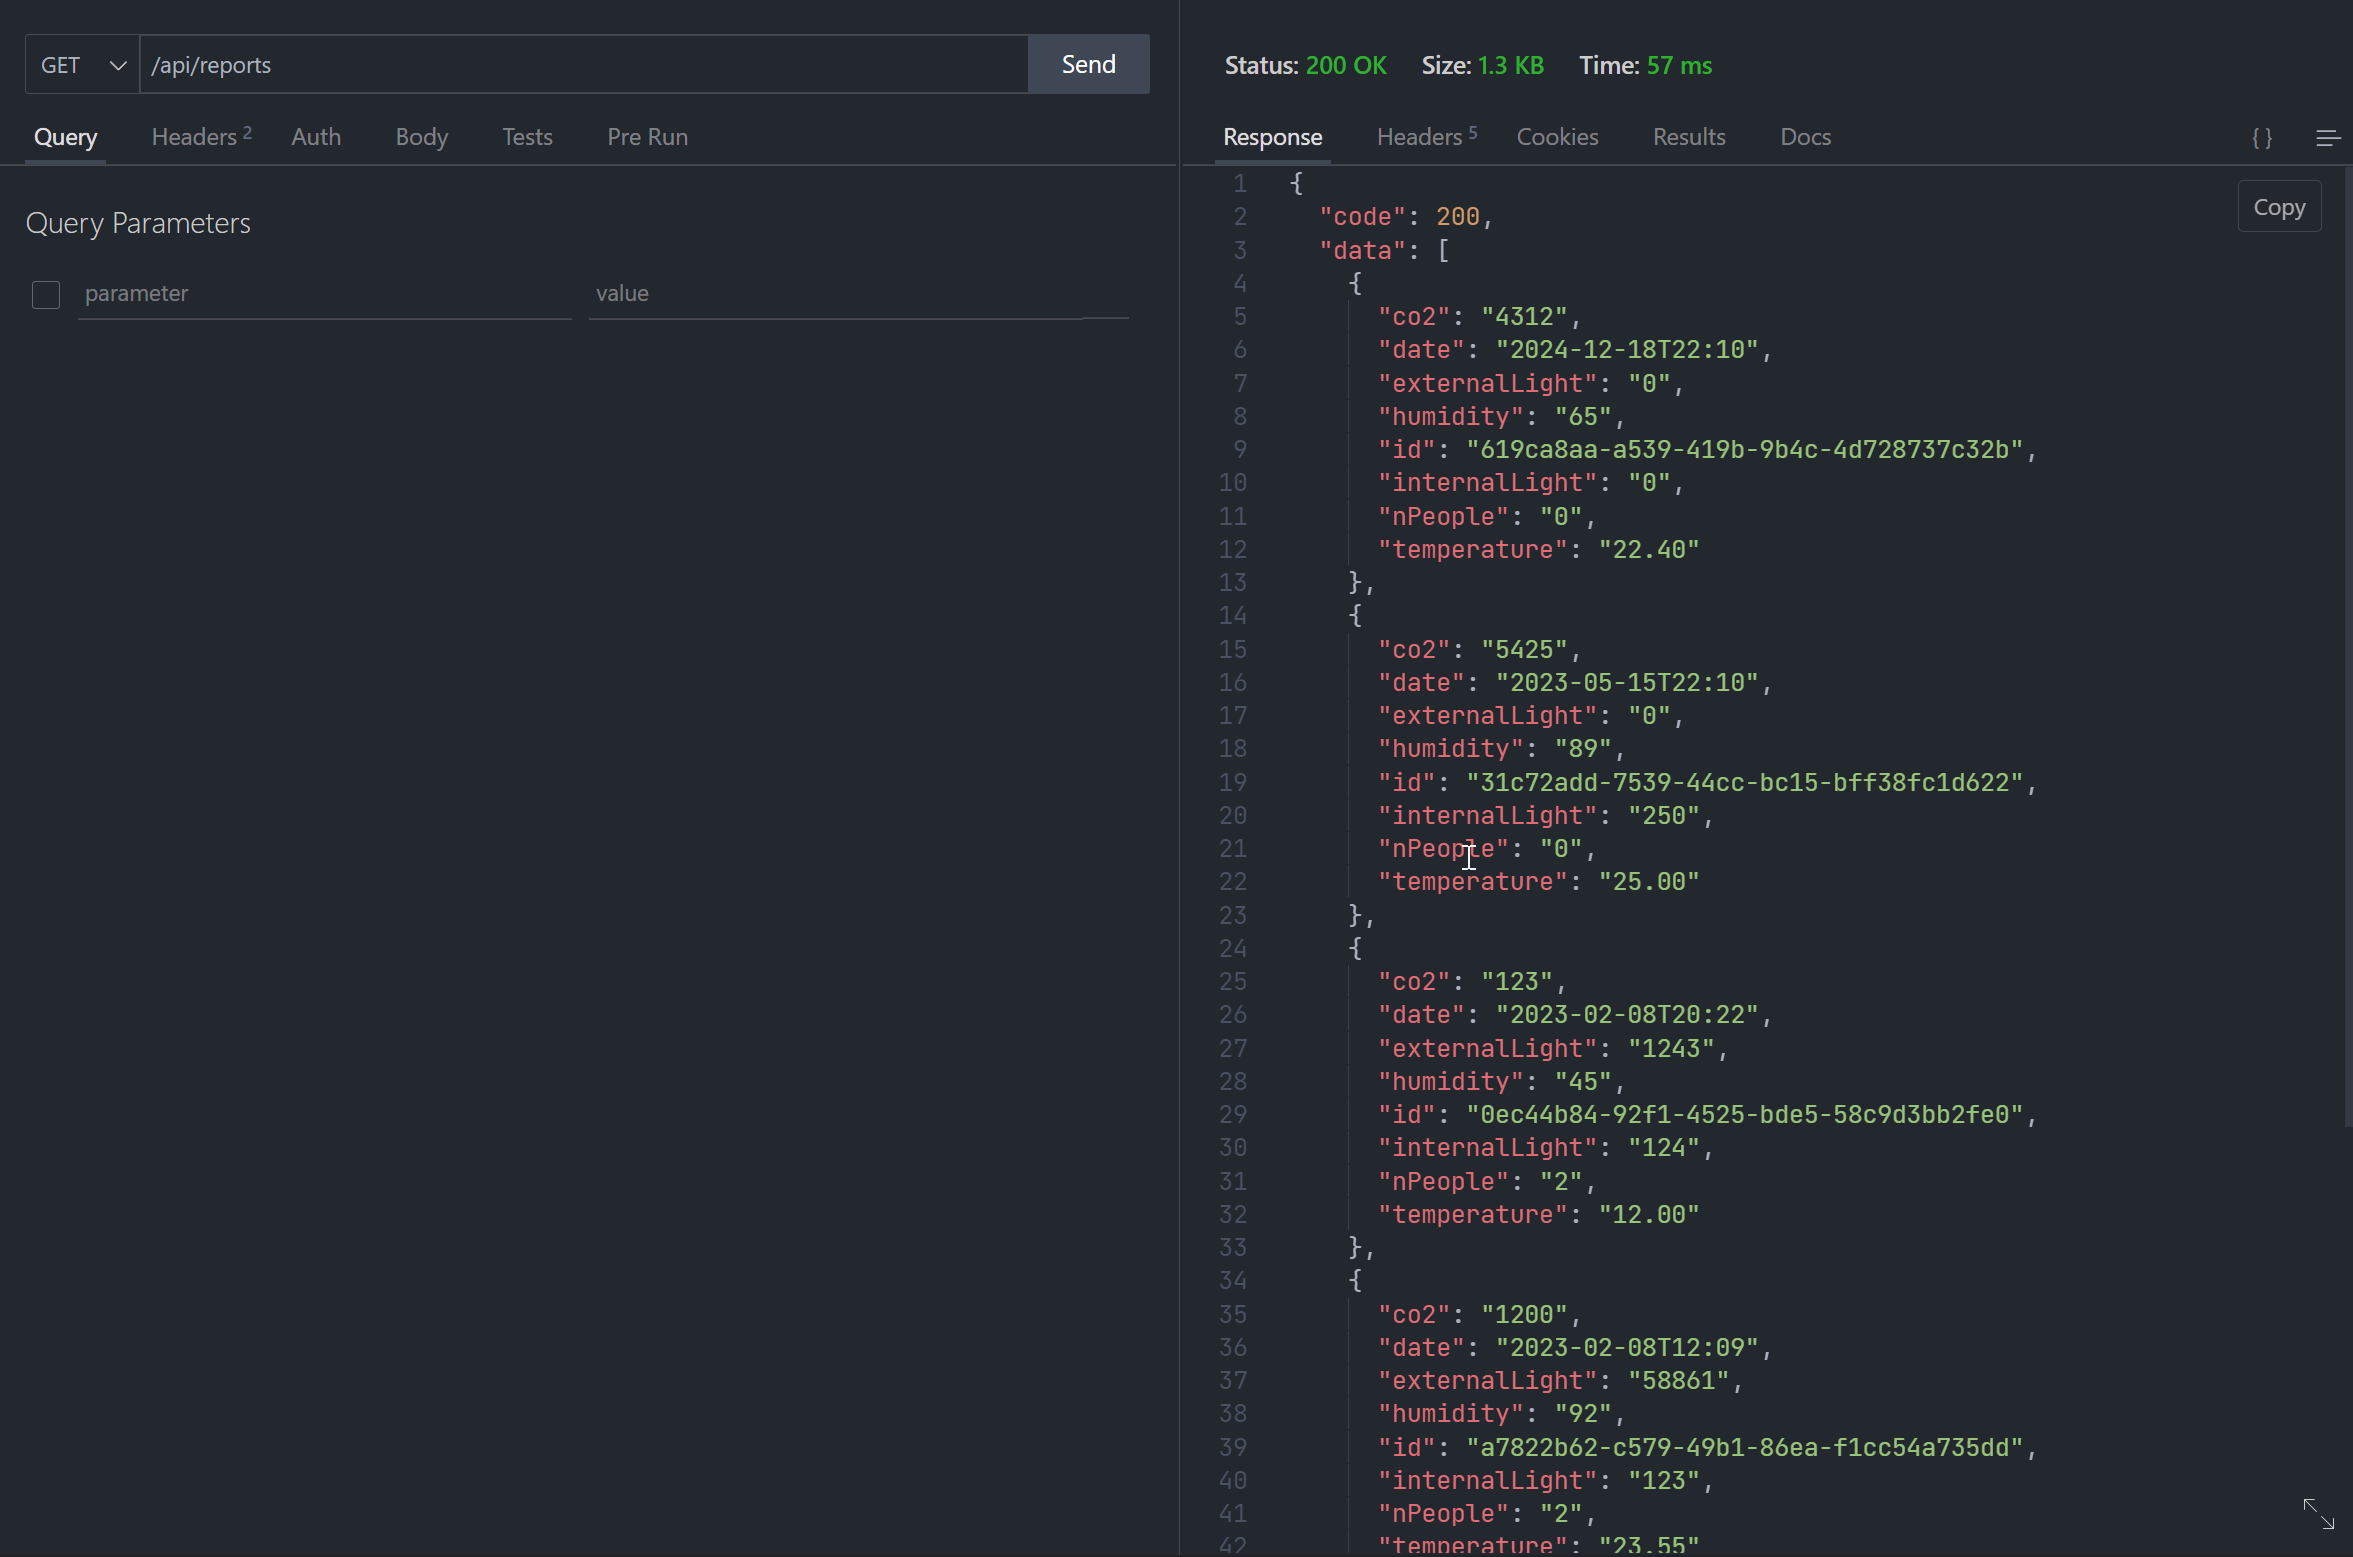
\includegraphics[scale=0.36]{figures/sample_api_response.png}
    \caption{Esempio risposta servizio Rest}
    \label{fig:rest_api_reponse}
\end{figure}


\vspace{8pt}
\subsubsection{Analisi PDF}\label{sec:domotics_pdf_analysis}
Per analizzare il PDF è stato necessario usare la libreria \href{https://pypdf2.readthedocs.io/en/3.0.0/}{pyPDF2}, che ha consentito la conversione del file creato dal \hyperref[sec:domotics_sensor]{sensore di CO2} in una stringa. Il team ha trovato varie difficoltà nell'individuare i dati all'interno della stringa ma dopo aver eliminato \emph{spazi} e \emph{caratteri di fine linea} il problema è stato risolto. Grazie a questa modifica si è riuscito ad individuare i dati cercando delle \emph{keywords} presenti in specifiche parti del PDF. In questo modo diviene possibile estrapolare vari dati dal PDF come data della misurazione, CO2, temperatura e umidità.

\vspace{8pt}
\subsubsection{Controlli domotici}\label{sec:domotics_domotics_server}
Per controllare le luci il server è stato connesso con \emph{Telnet} al server domotico dell'edificio. Dopo aver riscontrato alcune difficoltà nel trovare i comandi giusti e grazie alla guida di \emph{Amperia}, è stato possibile capire i giusti codici univoci assegnati a \emph{luci}, \emph{LIM}, \emph{tapparelle} e \emph{termostati} in un determinato ambiente, in maniera da controllarli tramite connessione \emph{Telnet}. Questa connessione ha fatto diventare l' \hyperref[sec:domotics_server]{HTTP Server} un \emph{client} per il server domotico in modo da controllare i dispositivi connessi.

\vspace{8pt}
\subsubsection{Analisi luce esterna}
La misurazione della luce interna è ricavata dal sensore del telefono tramite un'app ma la luce esterna non può essere ricavata direttamente da quest'ultima. La prima idea fu di aggiungere un \emph{Arduino} esternamente ma questo metodo non poteva essere applicato ad ogni possibile situazione ed edificio. La soluzione trovata è stata quella di fare chiamate ad una API esterna (\href{https://open-meteo.com/}{Open meteo}), la quale ritorna l'irradiazione solare di una posizione in $\frac{W}{m^2}$ che è poi convertita in $lux$ dal server.

\bigskip 
\section{NAO COME GUIDA A SOLAREDGE}\label{sec:solaredge_project}

Il progetto consiste in un interazione del NAO con il client del partner \emph{Amperia}, in cui vengoni richiesti i dettagli della struttura scelta, al fine di generare un progetto per una transizione solare con il sito Solaredge, rendendo la sostenibilità accessibile a tutti. Tutto ciò si suddivide in due fasi: una fase iniziale dove \hyperref[sec:solaredge_nao]{NAO} interroga il client e inserisce le risposte su un sito, richiedendo eventualmente un inserimento manuale quando non è in grado di controllare il sito. La seconda fase consiste in una spiegazione da parte del NAO di tutti i risultati ottenibili dal progetto e del suo relativo impatto ambientale. Il progetto è suddiviso in più elementi:\\

\begin{itemize}
    \item \hyperref[sec:solaedge_server]{Server HTTP}: un server Rest che comunica con il NAO e controlla il sito inserendo i dati richiesti
    \item \hyperref[sec:solaredge_nao]{NAO}: un robot umanoide che richiede i dettagli e invia le risposte al server che procederà all'analisi. Inoltre presenta a voce i risultati del progetto generato con il sito web Solaredge.
\end{itemize}

\begin{figure}[!htbp]
    \centering
    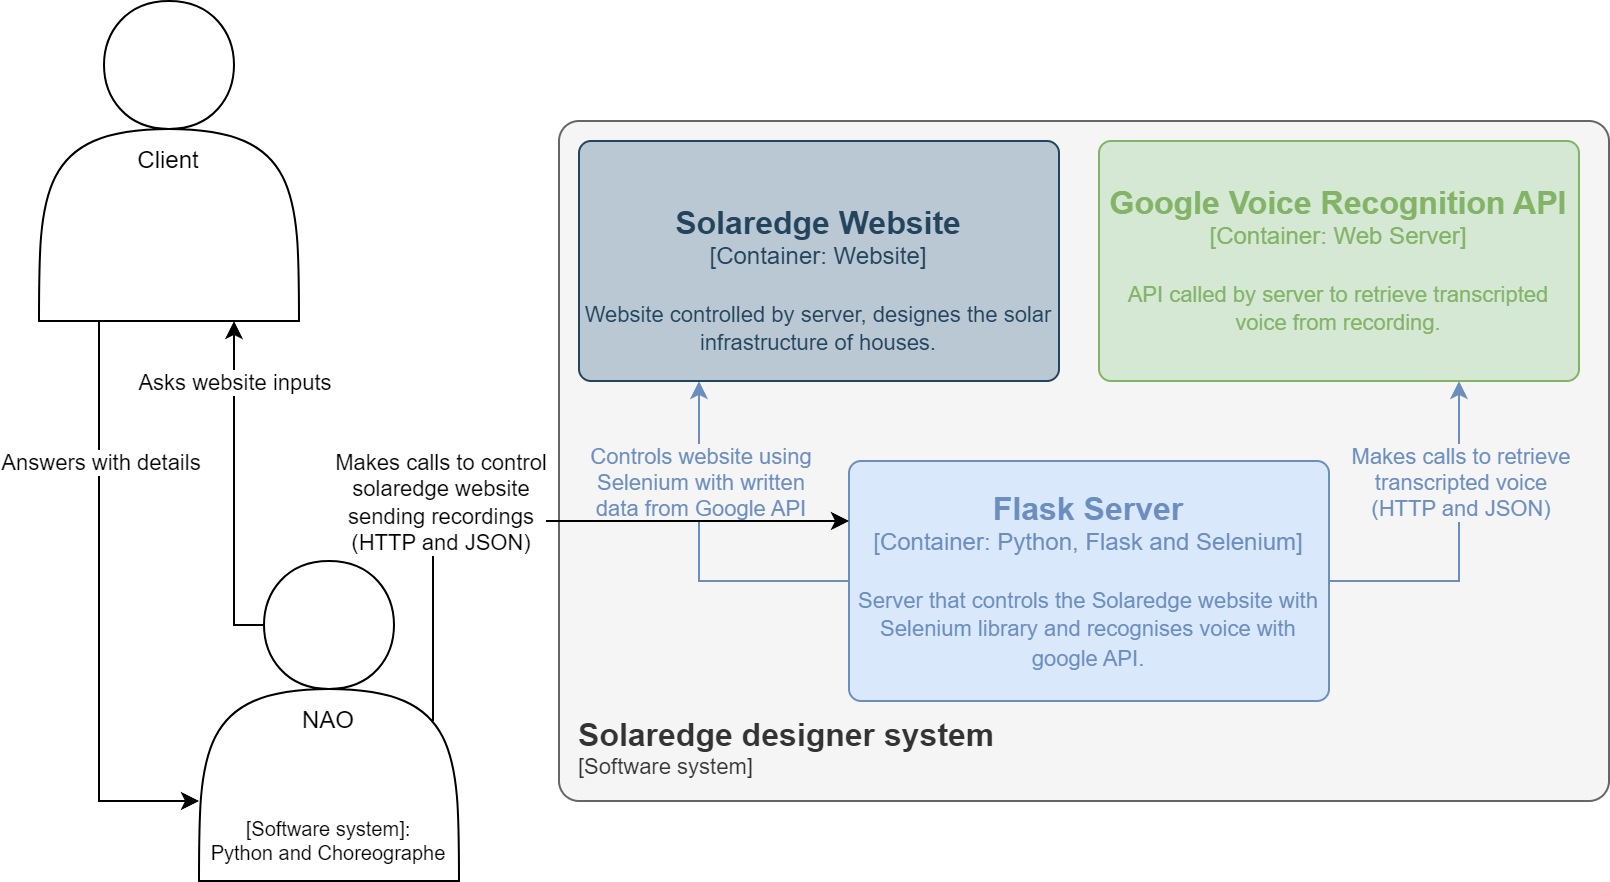
\includegraphics[scale=0.23]{figures/architecture_solaredge.png}
    \caption{Solaredge architecture}
    \label{fig:architecture_solaredge}
\end{figure}

\subsection{NAO}\label{sec:solaredge_nao}
NAO è la parte essenziale di questo progetto in quanto gestisce l'interazione con il cliente che dovrà configurare la sua installazione di pannelli solari. L'idea iniziale consisteva nell'aggiunta delle librerie necessarie per controllare il sito Solaredge direttamente come un \emph{pacchetto} Python del NAO. Tuttavia, vennero riscontrati gli stessi problemi del \hyperref[sec:domotics_server]{progetto precedente}: le librerie non potevano essere installate. La soluzione, fu quella di utilizzare un computer come \emph{server}, accedendo al sito direttamente da esso e rendendo dunque, la pagina web accessibile anche al cliente. Nell'interpretare i comandi del cliente il team ha incontrato un secondo problema: il riconoscimento vocale di NAO lavora solo con parole già definite in una lista ma, gli input dall'utente, possono essere potenzialmente infiniti. Il team ha quindi deciso di registrare la risposta con NAO ed inviare il file WAV al \hyperref[sec:solaedge_server]{server} affinchè possa essere analizzato. Quando il progetto è completo, il robot espone a voce i risultati del progetto generati dal sito web.

\vspace{12pt}
\subsection{HTTP Server}\label{sec:solaedge_server}
È il punto centrale in cui tutti i dati del progetto sono immagazzinati. È scritto in Python e comunica con NAO ricevendo le registrazioni vocali. Esso \hyperref[sec:solaredge_voice_recognition]{analizza le registrazioni} estraendo la trascrizione che viene poi \hyperref[sec:solaredge_website_control]{inserita nel sito Solaredge}. Include vari endpoints statici e dinamici per gestire i dati. È stato scritto in Python utilizzando \href{https://flask.palletsprojects.com/en/2.2.x/}{Flask}. Similarmente all'altro progetto, il \hyperref[sec:solaedge_server]{server} non è eseguito direttamente su NAO ma su un PC esterno, il che rende il codice flessibile aiutando l'utente ad inserire dati e ad accedere al sito.

\vspace{8pt}
\subsubsection{Rest API}\label{sec:solaredge_rest_api}
\textit{La documentazione per l'API può essere trovata \href{https://naonexus.notion.site/Solaredge-server-1bae2ae87b4d407b82f5a50bbfe3d87c}{qui}.}\\
\\Questo servizio Rest gestisce il traffico di dati dal NAO al server e nel senso opposto. Include vari endpoint e usa il protocollo HTTP. Inoltre i file WAV registrati da NAO sono trascritti ed inseriti nel sito web Solaredge.

\vspace{8pt}
\subsubsection{Riconoscimento vocale}\label{sec:solaredge_voice_recognition}
La trascrizione della voce viene fatta usando la libreria Python \href{https://pypi.org/project/SpeechRecognition/}{SpeechRecognition}, che utilizza il modello di \emph{Google} per il riconoscimento vocale e ritorna un testo a partire da un file audio. Il file passato a questa libreria è composto da due canali e include le registrazioni del microfono \emph{destro} e \emph{sinistro} del NAO.

\vspace{8pt}
\subsubsection{Solaredge website Control}\label{sec:solaredge_website_control}
\href{https://www.selenium.dev/documentation/}{Selenium} è una libreria Python che contiene numerose istruzioni, le quali permettono un'interazione diretta con un browser locale a scelta. Questo strumento può analizzare il codice HTML del sito e così facendo è in grado di selezionare ed interagire con specifici elementi grafici presenti nel codice stesso (come caselle di testo, liste, links etc.). Esso \emph{automatizza} sia l' \emph{estrazione} che l' \emph{importazione} dei dati, ottimizzando il processo e rendendolo più efficiente. Questa libreria è fondamentale per inserire le trascrizioni dei file audio estratti dalla conversazione tra \hyperref[sec:solaredge_nao]{NAO} e il cliente.

\newpage

\section{TEAM E AUTORI}\label{sec:team_authors}
Il team \emph{NaoNexus} è diviso in due sezioni: \emph{coding} e \emph{social}. I membri del team che hanno lavorato alla parte social del progetto si sono impegnati per rappresentare l'esperienza NaoNexus al meglio, creando e postando nuovi contenuti ogni giorno per evidenziare i progressi fatti dal gruppo durante questi mesi. Il sub-team social ha avuto un ruolo chiave nel rappresentare i progetti con video, immagini, reel e \href{https://www.tiktok.com/@naonexus}{TikTok}. Essi sono stati postati sui nostri social e sul \href{https://www.naonexus.altervista.org}{sito web} NaoNexus.

\bigskip
\noindent
Il gruppo coding si è occupato della parte di robotica, sviluppando il codice e lavorando con le tecnologie e metodologie pecedentemente presentate.\\

\subsection{GRUPPO CODING}

\noindent\emph{Riccardo Antonelli - Team Leader}\\
\emph{Francesco Bernardi}\\
\emph{Elisa D'Iseppi}\\
\emph{Filippo Buso}\\
\emph{Edoardo Polfranceschi}\\

\bigskip

\subsection{GRUPPO SOCIAL}

\noindent\emph{Alberto Rubini - Team Leader}\\
\emph{Davide Masini}\\
\emph{Antonio Galati}\\
\emph{Arianna Antonelli}\\


\begin{figure}[b]
    \centering
    
\includegraphics[scale=0.04]{figures/logo.png}
    \label{fig:logo_con_scritta1}
\end{figure}


%\vspace{70pt}
%\listoffigures
\end{document}